\documentclass[twocolumn,english]{IEEEtran}
\usepackage[T1]{fontenc}
\usepackage{babel}
\usepackage{amsthm}
\usepackage{amsmath}
\usepackage{graphicx}
\usepackage[unicode=true,
 bookmarks=true,bookmarksnumbered=true,bookmarksopen=true,bookmarksopenlevel=1,
 breaklinks=false,pdfborder={0 0 0},backref=false,colorlinks=false]
 {hyperref}
\usepackage{bm}
\usepackage{amsmath}
\usepackage{amssymb}
\usepackage{natbib}
\usepackage{array}
\usepackage{calc}
\usepackage{booktabs}
\newcolumntype{W}{>{\centering\arraybackslash}m{25mm}}
\newcolumntype{L}{>{\centering\arraybackslash}m{15mm}}


\hypersetup{
 pdftitle=  {Lenses, Mirrors, and Ray Tracing},
 pdfauthor= {Zack Garza},
 pdfpagelayout=OneColumn, pdfnewwindow=true, pdfstartview=XYZ, plainpages=false}

\makeatletter


%%%%%%%%%%%%%%%%%%%%%%%%%%%%%% Textclass specific LaTeX commands.
 % protect \markboth against an old bug reintroduced in babel >= 3.8g
 \let\oldforeign@language\foreign@language
 \DeclareRobustCommand{\foreign@language}[1]{%
   \lowercase{\oldforeign@language{#1}}}
\theoremstyle{plain}
\newtheorem{thm}{\protect\theoremname}
\theoremstyle{plain}
\newtheorem{lem}[thm]{\protect\lemmaname}

%%%%%%%%%%%%%%%%%%%%%%%%%%%%%% User specified LaTeX commands.
% for subfigures/subtables
\ifCLASSOPTIONcompsoc
\usepackage[caption=false,font=normalsize,labelfont=sf,textfont=sf]{subfig}
\else
\usepackage[caption=false,font=footnotesize]{subfig}
\fi

\makeatother
\providecommand{\lemmaname}{Lemma}
\providecommand{\theoremname}{Theorem}
\setcounter{topnumber}{2}
\setcounter{bottomnumber}{2}
\setcounter{totalnumber}{4}
\renewcommand{\topfraction}{0.85}
\renewcommand{\bottomfraction}{0.85}
\renewcommand{\textfraction}{0.15}
\renewcommand{\floatpagefraction}{0.7}
\usepackage{float}
\begin{document}

\title{Lenses, Mirrors, and Ray Tracing}


\author{Zack Garza}


\IEEEspecialpapernotice
{Physics 215L \\
Effective Date of Report: 23 April, 2014 }


\markboth{Lenses, Mirrors, and Ray Tracing}{Zack Garza}

\maketitle

\tableofcontents


\section{Theory}

\section{Results}

\subsection{Focal Length Measurements}

\subsubsection{Distant Object Method}

The lenses were placed a large distance from the image, and the image distances were measured. The object distance was taken to be infinite, and thus equal to the focal length by the expression
\begin{align}
	\frac{1}{f} &= \frac{1}{p} + \frac{1}{q} \notag \\
	&= \frac{1}{\infty} + \frac{1}{q} \notag \\
	&= \frac{1}{1} \notag \\
	\Rightarrow f &= p.
\end{align}

\begin{table}[H]
	\caption{Focal Length Measurements}
	\label{tb:focal_length}
	\centering
	\begin{tabular}{@{}lllll@{}}
	\toprule
	Element	& Image Distance ($\pm$ .2 cm) 	& Focal Length ($\pm$ .2 cm)  \\ \midrule
	A 		& 20.2			& 20.2 	\\
	B 		& 13.1 			& 13.1 	\\
	Mirror 	& 7.4  			& 7.4 	\\
	C 		& 5.5			& 9.5 	\\ \bottomrule
	\end{tabular}
\end{table}

\subsubsection{Near Object Method}

Ordered pairs were obtained for image and object distance for Lens A, and their focal length was calculated from
\begin{equation}
	\frac{1}{f} = \frac{1}{p} + \frac{1}{q}.
\end{equation}

\begin{table}[H]
	\caption{Near Object Method for Lens A}
	\label{tb:nearobj}
	\centering
	\begin{tabular}{@{}lll@{}}
	\toprule
	$p$ (cm)      & $q$ (cm)     & $f$ (cm)     \\ \midrule
	115.00    	& 23.35 	& 19.41 \\
	109.45 		& 23.60  	& 19.41 \\
	105.00    	& 24.20  	& 19.67 \\
	95.00     	& 25.35 	& 20.01 \\
	90.40   	& 26.38 	& 20.42 \\
	85.00     	& 27.20  	& 20.61 \\
	78.00     	& 31.49 	& 22.43 \\
	75.00     	& 33.85 	& 23.32 \\ \midrule
	$f$ Average: 20.7 cm $\pm$ 0.5 cm \\ \bottomrule
	\end{tabular}
\end{table}
The plot of this data is shown in Figure~\ref{fig:1q1p} on Page~\pageref{fig:1q1p}.


\subsection{Two-Lens System}

\begin{table}[H]
\caption{Two-Lens System Measurements}
\label{tb:twolens}
\centering
\begin{tabular}{@{}lll@{}}
\toprule
 Object Distance  (cm) & $D$ (cm) & Image Distance (cm)  \\ \midrule
 35.0 & 20.0  & 36.1 \\ \bottomrule
\end{tabular}
\end{table}

The image is inverted, and is smaller than the source.

\subsection{Mirror-Lens System}
\textit{Observations:} An inverted image appears that is slightly smaller than the original.

\onecolumn

\begin{figure}[h!]
	\begin{centering}
	\begin{center}
	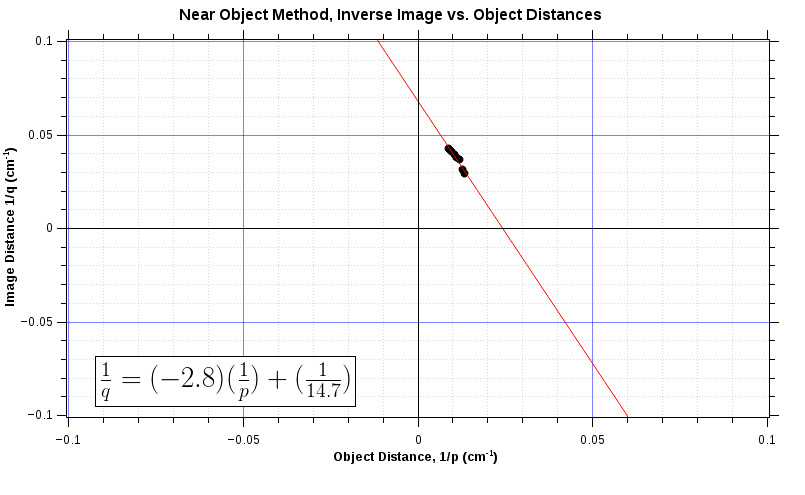
\includegraphics[width=\linewidth]{./Images/Graph1.png}
	\caption{The inverse of the Y-intercept is 14.5cm, while that of the X-intercept is 41.1cm.}
	\label{fig:1q1p}
	\end{center}
	\par\end{centering}
\end{figure}

\twocolumn
\section{Results}

\subsection{Part 1: Focal Length Measurements}
\begin{enumerate}
	\item \textit{What is the value of $f_A$ from the graph?}

	$1/f_A$ corresponds to the point at which $1/p$ is zero, which corresponds to an infinite object distance. Taking the inverse of the y-intercept from the graph yields
	\begin{align*}
		f_A = 14.7 \text{cm}.
	\end{align*}

	\item \textit{What do the values in the second quadrant represent?}

	Since $1/p$ is negative in this quadrant, the values correspond to negative object distances. Physically, this represents the image location when the object is virtual and located behind the lens. Similarly, the values below the y-axis correspond to virtual images.

	\item \textit{How does the value of $f_A$ from the distant object method compare to that of the near object method? How good is the distant object method?}

	Both methods agreed fairly well, resulting in a percent difference of only \underline{2.4 \%}.

	Each method has its own strengths and weakness. The uncertainty due to image blurriness in the distant-object method was smaller than the statistical error from the near-object method measurements, however the distant-object method required a more subjective definition of what constituted a ``clear'' image. The near-object images were easily distinguishable, and increasing the number of data points in the near-object method could lower the overall error. Regardless, the distant object method turned out to be a very good approximation.

	\textit{What is the difference between the values from the distant object method and from the graph?}

	These values were dissimilar, resulting in a difference of \underline{32\%}. Error may arise from the goodness of the fit and rounding errors, however inspection of the original data points showed that the values had a wide spread and were only approximately linear to begin with.
\end{enumerate}

\subsection{Part 2: Two-Lens System}
\begin{enumerate}
	\item \textit{Can this lens system be used to correct myopia, or hyperopia? Explain why and how.}

	This lens system can be used to correct myopia, or nearsightedness. Since the eye can be modeled as a converging lens, the diverging lens is the key element in this correction. For a myopic person, the focal length of the eye is too short, so the rays fall slightly short of the retina. This produces a blurred image, and shifts the far point closer than usual. A diverging lens with the proper focal length serves to bring objects located far away to the eye's natural far point by creating a virtual image at that point. This causes the rays from the image to properly converge on the retina, producing a sharp image.

	\item \textit{Suppose an object is placed to the left of a converging lens, farther than the focal point, and that an image is formed at $q_1$. Then suppose a diverging lens is placed to the right of the converging lens, between the lens and $q_1$. Is the observed image real or virtual? Is it upright or inverted? Why?}

	In this case, the image could be either real or virtual -- it depends on how close the closer the diverging lens is to the image, and the size of its focal length.

	Since increasing the focal length has the same effect as moving the lens closer to the image, consider the possible outcomes for just one of these cases. If the diverging lens is very close to the converging lens, then the light from the image will be scattered and not converge on a real location. The only image seen will be from tracing the diverging light rays backwards, so the image will appear to the \textit{left} of the diverging lens in this case. It will be upright, since the original image was inverted, and back-tracing the rays flips the image axis.

	However, as the lens is moved toward the object (or the focal length is increased), the rays emanating from the diverging lens begin to converge. The virtual image goes to infinity on the left, and a real image approaches from infinity on the right. If the diverging lens is far enough away that the rays from the converging lens have converged ``enough'', the rays are not completely diverged and produce a second, inverted, real image.
\end{enumerate}

\subsection{Part 3: Mirror-Lens System}
\begin{enumerate}
	\item \textit{Discuss the number of images that would be observed if the object was placed farther than the mirror's focal length.}

	If the object is moved farther than the mirror's focal length, a second image can be seen. It is a virtual image produced by back-tracing the rays between the lens and the mirror, and can be slightly larger than the first image.

	If the object is moved close to the lens, the first image goes infinitely to the right as the rays diverge, a third image can be seen approaching from infinity on the left as the rays begin to converge again. This image is real, and upright, and can possible be magnified depending on the distances and focal lengths.

	And while it does not appear on the screen, a fourth, inverted real image will also occur between the object and the mirror.
\end{enumerate}


\appendices{}


%\bibliographystyle{plain}
%\bibliography{physbib}

\end{document}